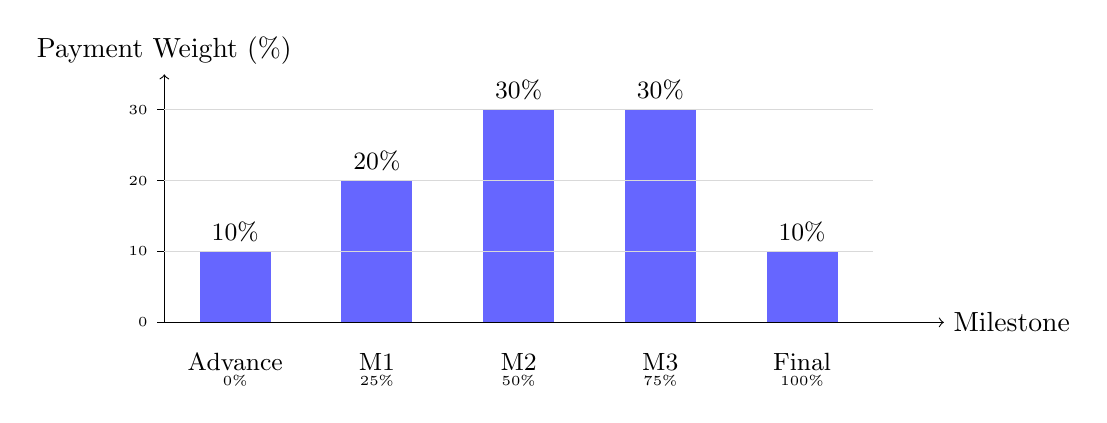
\begin{tikzpicture}[scale=0.9]
    % Simple bar chart using basic TikZ
    \draw[->] (0,0) -- (0,3.5) node[above] {Payment Weight (\%)};
    \draw[->] (0,0) -- (11,0) node[right] {Milestone};
    
    % Bars (height scaled: 1 unit = 10%)
    \fill[blue!60] (0.5,0) rectangle (1.5,1.0);
    \node[above] at (1,1.0) {\small 10\%};
    \node[below] at (1,-0.3) {\small Advance};
    \node[below, font=\tiny] at (1,-0.6) {0\%};
    
    \fill[blue!60] (2.5,0) rectangle (3.5,2.0);
    \node[above] at (3,2.0) {\small 20\%};
    \node[below] at (3,-0.3) {\small M1};
    \node[below, font=\tiny] at (3,-0.6) {25\%};
    
    \fill[blue!60] (4.5,0) rectangle (5.5,3.0);
    \node[above] at (5,3.0) {\small 30\%};
    \node[below] at (5,-0.3) {\small M2};
    \node[below, font=\tiny] at (5,-0.6) {50\%};
    
    \fill[blue!60] (6.5,0) rectangle (7.5,3.0);
    \node[above] at (7,3.0) {\small 30\%};
    \node[below] at (7,-0.3) {\small M3};
    \node[below, font=\tiny] at (7,-0.6) {75\%};
    
    \fill[blue!60] (8.5,0) rectangle (9.5,1.0);
    \node[above] at (9,1.0) {\small 10\%};
    \node[below] at (9,-0.3) {\small Final};
    \node[below, font=\tiny] at (9,-0.6) {100\%};
    
    % Y-axis labels
    \foreach \y in {0,10,20,30} {
        \draw (0,\y/10) -- (-0.1,\y/10) node[left, font=\tiny] {\y};
    }
    
    % Grid
    \foreach \y in {1,2,3} {
        \draw[gray!30] (0,\y) -- (10,\y);
    }
\end{tikzpicture}
